\section{Harness Composition}
\label{sec:method-foundry}

The gap identified in Section~\ref{sec:related-harness-eng} is the absence of an infrastructure layer that exposes the harness as a typed, substitutable entity. Primitive libraries leave composition to application code, orchestrators expose a fixed set of patterns, and product harnesses are opaque end-to-end. Without a compositional substrate, every behavioral change or cross-team handoff requires re-implementation. \ProjectName addresses this via a unified design principle: the harness is a first-class value, the processor is a typed atomic component, and composition proceeds via processor insertion at typed hook points. We formalize the harness (Section~\ref{sec:foundry-object}), its building block, the processor (Section~\ref{sec:foundry-processor}), and the nine-dimensional processor taxonomy (Section~\ref{sec:foundry-taxonomy}). Definitions are intentionally concise: their role is to establish the vocabulary and expose the edit surface on which harness evolution (Section~\ref{sec:method-aegis}) operates.

\begin{table}[!htbp]
\centering
\small
\begin{tabular}{lll}
\toprule
Hook & Event type & Permitted modifications \\
\midrule
\texttt{task\_start}    & \texttt{TaskStartEvent}     & system prompt \\
\texttt{step\_start}    & \texttt{StepStartEvent}     & structural history edits \\
\texttt{before\_model}  & \texttt{BeforeModelEvent}   & last user content; one user-message append \\
\texttt{after\_model}   & \texttt{ModelResponseEvent} & response content, tool calls \\
\texttt{before\_tool}   & \texttt{ToolCallEvent}      & tool input, approval flag \\
\texttt{after\_tool}    & \texttt{ToolResultEvent}    & tool result \\
\texttt{step\_end}      & \texttt{StepEndEvent}       & read-only \\
\texttt{task\_end}      & \texttt{TaskEndEvent}       & read-only \\
\bottomrule
\end{tabular}
\caption{Hook points and their permitted modifications.}
\label{tab:hook-points}
\end{table}

\subsection{The Harness as a First-Class Object}
\label{sec:foundry-object}

A harness in \ProjectName is the pair $\mathcal{H} = (\mathcal{M}, \mathcal{C})$, where $\mathcal{M}$ is a model configuration and $\mathcal{C}$ is a harness configuration. The two address disjoint concerns: $\mathcal{M}$ records \textit{which} model serves which role (\texttt{main}, \texttt{judge}, \texttt{evaluator}) and the fallback policy for each role; $\mathcal{C}$ records \textit{how} the agent behaves independently of model identity. They combine into an executable agent via \texttt{agent = model\_config.agentic(harness\_config)}: an agent in \ProjectName is a processor pipeline bound to a model, both independently substitutable.

The harness configuration itself decomposes as $\mathcal{C} = (\mathbf{P}, \mathbf{S})$. $\mathbf{P} : \mathcal{H}\!\mathit{ook} \to \mathrm{List}[\mathit{Processor}]$ is a hook-indexed list of processors, where $\mathcal{H}\!\mathit{ook}$ is the eight-element set of lifecycle events in Table~\ref{tab:hook-points}. $\mathbf{S}$ is a fixed set of orthogonal \textit{slot resources}: tool registry, tracer, workspace, sandbox provider, and plugin list. Slots are singletons, shared across all processors in a configuration; processor state is instance-private. $\mathbf{P}$ implements all per-step behavior; $\mathbf{S}$ houses the shared infrastructure that processors depend on but do not own.

We call $\mathcal{C}$ a first-class object because it is independently serializable, comparable, hashable, and substitutable. Two agents sharing $\mathcal{C}$ but differing in $\mathcal{M}$ execute the same processor pipeline, with behavior differing only in model responses; two agents sharing $\mathcal{M}$ but differing in $\mathcal{C}$ are behaviorally distinct. This reification is the precondition for programmatic evolution (Section~\ref{sec:method-aegis}).

\subsection{The Processor Abstraction}
\label{sec:foundry-processor}

Every per-step behavior in \ProjectName is implemented as a \textit{processor}, an object satisfying the protocol \texttt{async def process(self, event: Event) -> AsyncIterator[Event]}. A processor consumes one event and yields zero or more, producing exactly one of five outcomes: pass-through (yield unchanged), transform (yield modified), split (yield multiple same-type events, processed independently downstream), intercept (yield nothing, blocking propagation), or interrupt (raise an exception, which halts the loop). This restricted interface enables compositionality: every processor at a given hook consumes and yields the same event type, so processors compose by sequential application and can be inserted or removed without affecting type correctness of the surrounding pipeline.

As listed in Table~\ref{tab:hook-points}, processors attach to one of eight hook points emitted by the run loop. The run loop validates hook contracts after each invocation: a violation (e.g., modifying a read-only field) raises an exception immediately rather than silently propagating corrupted state. Each processor carries three class-level metadata fields that govern composition: \texttt{\_singleton\_group} names a mutual-exclusion class, ensuring at most one processor per group; \texttt{\_order} is an ordering hint within a hook (with constants \texttt{PRE}, \texttt{NORMAL}, \texttt{POST}); and \texttt{\_after} is a list of soft dependencies on other singleton groups.

This design makes harness evolution a first-class operation: AEGIS can insert a new processor at a specific hook, replace an existing one by matching its singleton group, or remove a processor entirely---all without touching other processors at the same or different hooks. Because the type contract (input event type $=$ output event type) is enforced per-hook, any such substitution preserves the well-typedness of the overall pipeline. The metadata fields further constrain composition: \texttt{\_singleton\_group} prevents conflicting duplicates, and \texttt{\_order} ensures that newly inserted processors interact predictably with existing ones. These guarantees are the mechanism by which variant isolation (Section~\ref{sec:aegis-ensemble}) operates---each variant differs only in which processors occupy which hooks, and the type system ensures that no variant can silently violate the pipeline contract during evolution.

\subsection{The Nine-Dimensional Taxonomy}
\label{sec:foundry-taxonomy}

We organize the behavioral space along nine dimensions: \textit{model selection} (D1) decides which model serves which role; \textit{context assembly} (D2) determines what is presented to the model at each step; \textit{memory management} (D3) governs what carries across steps and sessions; \textit{tool ecosystem} (D4) controls which tools the agent can invoke; \textit{execution environment} (D5) determines where tool-induced side-effects materialize; \textit{evaluation and reward} (D6) specifies how outcomes are judged; \textit{control and safety} (D7) enforces rules that keep the agent from looping, overspending, or drifting from intent; \textit{observability} (D8) records each event, model call, and tool invocation; and the \textit{training bridge} (D9) converts execution trajectories into reinforcement-learning records. Figure~\ref{fig:aegis-loop} illustrates the full taxonomy along with representative processors and the hooks at which they typically attach in a standard configuration.

In practice, AEGIS edits span all nine dimensions during evolution: D2 (context assembly) and D4 (tool ecosystem) are the most frequent edit targets (Section~\ref{sec:exp-main}), while D8 (observability) provides the trace substrate on which AEGIS itself reasons, and D9 (training bridge) supplies trajectory records for co-evolution (Section~\ref{sec:method-coevolution}), closing the optimization loop.



% \begin{figure}[!htbp]
%   \centering
%   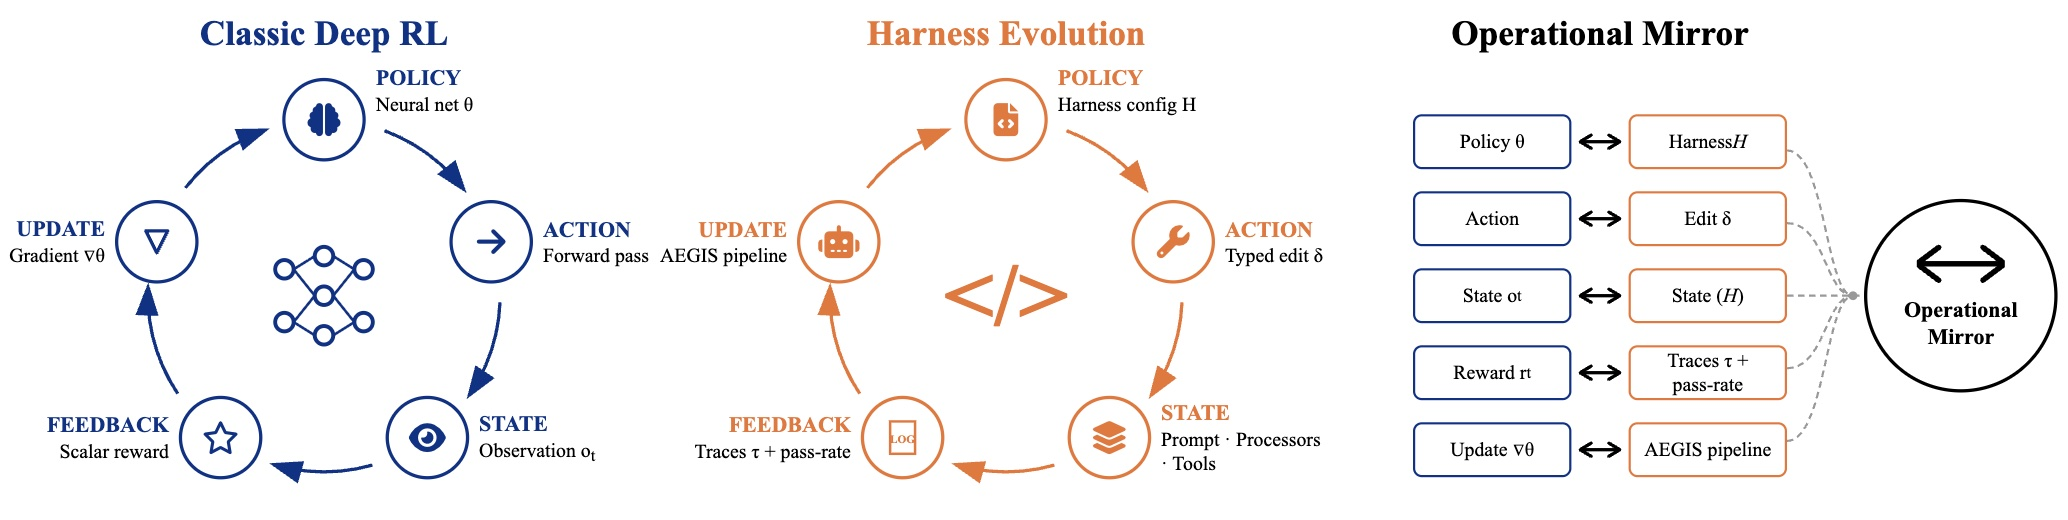
\includegraphics[width=\columnwidth]{images/Mirro.jpg}
%   \caption{The operational mirror between reinforcement learning and symbolic harness evolution. Each RL concept maps onto a concrete AEGIS mechanism, converting familiar RL pathologies into actionable design requirements.}
%   \label{fig:operational-mirror}
% \end{figure}


\begin{table}[!htbp]
\centering
\small
\begin{tabular}{lll}
\toprule
\textbf{RL concept} & \textbf{Symbolic-space dual} & \textbf{AEGIS realization} \\
\midrule
Policy $\pi$ & Harness-update procedure $\pi_{\mathrm{evo}}$ & Four-stage pipeline (Section~\ref{sec:aegis-arch}) \\
State $s_t$ & $(\mathcal{H}_t, \mathcal{T}_t)$ & Harness configuration + trace store \\
Action $a_t$ & Typed harness edit & Builder operation + change manifest \\
Feedback & Trace $\tau$ + verifier score $r$ & Observability layer \\
Update & $\mathcal{H}_{t+1} \leftarrow U(\widetilde{\mathcal{H}}_{t}, \mathcal{T}_t, r_t)$ & Deterministic acceptance gate \\
\bottomrule
\end{tabular}
\caption{Operational mirror: RL concepts and their symbolic-space duals in AEGIS.}
\label{tab:operational-mirror}
\end{table}


\section{Harness Adaptation}
\label{sec:method-aegis}

The composition layer (Section~\ref{sec:method-foundry}) provides a typed, substitutable harness; as illustrated in Figure~\ref{fig:aegis-loop}, AEGIS is the system that evolves it. The key insight is that harness evolution maps structurally onto reinforcement learning in a symbolic space: harness configurations are states, typed edits are actions, and execution traces plus verifier scores constitute feedback. This mapping is predictive: it identifies three failure modes analogous to known RL pathologies (reward hacking, catastrophic forgetting, under-exploration) that motivate AEGIS's architectural defenses and are empirically confirmed in Section~\ref{sec:exp-failure}.

We formalize the correspondence (Section~\ref{sec:aegis-mirror}), analyze the pathologies it predicts (Section~\ref{sec:aegis-pathologies}), derive the four-stage pipeline as a defense architecture (Section~\ref{sec:aegis-arch}), present the adaptation loop (Section~\ref{sec:aegis-loop}), and introduce variant isolation for stable multi-variant evolution (Section~\ref{sec:aegis-ensemble}).



\begin{figure}[!htbp]
  \centering
  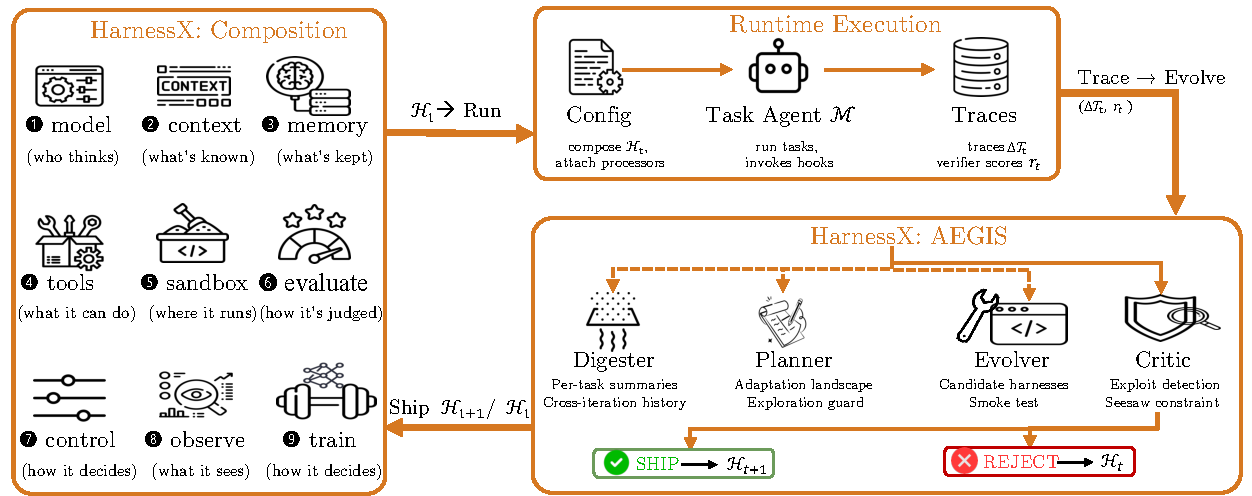
\includegraphics[width=\columnwidth]{images/Harness_Evolution.pdf}
  \caption{The AEGIS evolution loop. A single meta-agent $\mathcal{M}$ drives all four stages (Digester, Planner, Evolver, Critic), selectively invoking each based on whether sufficient signal exists to continue. A deterministic gate ships or rejects the candidate edit.}
  \label{fig:aegis-loop}
\end{figure}

\subsection{The Operational Mirror}
\label{sec:aegis-mirror}

We formalize harness evolution as an MDP over symbolic artifacts. Table~\ref{tab:operational-mirror} summarizes the mapping; we first state three definitions that ground the correspondence.

\paragraph{Definition 1 (Harness Configuration).}
A harness configuration is a tuple $\mathcal{H} = (c_1, c_2, \ldots, c_9)$, where each $c_i \in \mathcal{C}_i$ instantiates one of the nine behavioral dimensions (Section~\ref{sec:foundry-taxonomy}): model selection ($c_1$), context assembly ($c_2$), memory management ($c_3$), tool ecosystem ($c_4$), execution environment ($c_5$), evaluation and reward ($c_6$), control and safety ($c_7$), observability ($c_8$), and training bridge ($c_9$). Each $\mathcal{C}_i$ is the set of valid processor configurations for dimension $i$, constrained by hook-type contracts and singleton-group exclusion (Section~\ref{sec:foundry-processor}).

\paragraph{Definition 2 (Harness Edit).}
A harness edit is a function $e: \mathcal{H} \to \mathcal{H}$ that modifies one or more dimensions while preserving type contracts. The action space $\mathcal{E}$ is \textit{discrete but open-ended}: each edit is a code-level artifact (new processor source, modified prompt template, reconfigured tool registry, or control-flow rewrite) generated by the meta-agent LLM, not selected from a pre-enumerated set. Combinatorial explosion is managed not by exhaustive search but by the LLM's generative capacity---the Planner proposes edits from trace-grounded hypotheses---and by type constraints that prune invalid compositions at generation time.

\paragraph{Definition 3 (Operational Mirror).}
The operational mirror is the tuple $(\mathcal{H}, \mathcal{E}, \mathcal{R}, \mathcal{T})$, where $\mathcal{H}$ is the harness-configuration space (states), $\mathcal{E}$ is the code-level edit space (actions), $\mathcal{R}: \mathcal{H} \times \mathcal{E} \to \mathbb{R}$ maps a configuration--edit pair to a scalar reward (verifier scores aggregated over an adaptation batch), and $\mathcal{T}$ is the trace store that provides structured feedback beyond the scalar signal. This tuple forms an MDP at the harness level: harness configurations are states, typed edits are actions, execution traces plus verifier scores constitute feedback, and a deterministic acceptance gate governs state transitions.

\paragraph{MDP instantiation.}
Let $\mathcal{H}_t$ denote the harness configuration at iteration $t$ (the model $\mathcal{M}$ is fixed throughout evolution), and let
$\mathcal{T}_t$ denote the trace store accumulated from all previous executions. We
define the symbolic state as $s_t=(\mathcal{H}_t,\mathcal{T}_t)$. A harness-update
policy $\pi_{\mathrm{evo}}$ selects an action
$a_t \sim \pi_{\mathrm{evo}}(\cdot \mid s_t)$, where $a_t \in \mathcal{E}$ is a code-level edit drawn
from the builder algebra. Applying this edit yields a candidate harness
$\widetilde{\mathcal{H}}_{t}=a_t(\mathcal{H}_t)$. Running the candidate on an adaptation batch (with the fixed model $\mathcal{M}$) produces new traces $\Delta\mathcal{T}_t$ and per-task verifier scores $r_t$. A deterministic acceptance operator
$U(\widetilde{\mathcal{H}}_{t}, \mathcal{T}_t, r_t)$ then either commits the candidate
($\mathcal{H}_{t+1}=\widetilde{\mathcal{H}}_{t}$) or rejects it
($\mathcal{H}_{t+1}=\mathcal{H}_t$), enforcing the seesaw constraint: the candidate must not regress any previously solved task recorded in $\mathcal{T}_t$. In both cases, the trace store grows:
$\mathcal{T}_{t+1}=\mathcal{T}_t \cup \Delta\mathcal{T}_t$.

This MDP operates at the harness level: within a single task, $\mathcal{H}_t$ (together with the fixed $\mathcal{M}$) determines the agent's behavior; across iterations, the harness-update policy $\pi_{\mathrm{evo}}$ modifies the harness. AEGIS realizes $\pi_{\mathrm{evo}}$ as a four-stage pipeline (Digester, Planner, Evolver, Critic) that maps $s_t$ to candidate edits through trace compression, adaptation planning, edit generation, and candidate assessment.





\subsection{Pathologies in Symbolic Space}
\label{sec:aegis-pathologies}

The mirror is not merely an analogy; it converts reinforcement-learning concepts into design requirements. We refer to three well-documented failure modes in RL, namely reward hacking~\cite{guo2025deepseek}, catastrophic forgetting~\cite{kirkpatrick2017overcoming}, and under-exploration~\cite{ladosz2022exploration}, collectively as \textit{RL pathologies}. Once harness adaptation is cast as an MDP over symbolic artifacts, these pathologies reappear in amplified form, shaped by two properties of the symbolic setting: (1)~a language-model evolver can construct structured exploits that numerical parameter perturbations cannot express, and (2)~edits to shared components propagate non-locally through the harness. Each pathology below motivates a corresponding architectural defense in Section~\ref{sec:aegis-arch}.


\paragraph{Reward hacking.}
In standard RL, reward hacking~\cite{guo2025deepseek} exploits loopholes in the reward signal without genuine task completion. Symbolic harness evolution amplifies this risk because the evolver can target the verification protocol directly: embedding benchmark answers into prompts, exploiting format regularities in the verifier, or introducing a processor that rewrites outputs to match verifier expectations.

\paragraph{Catastrophic forgetting.}
Catastrophic forgetting~\cite{kirkpatrick2017overcoming} occurs when improving performance on one region of the task distribution harms another. In symbolic harness evolution, an edit that repairs failure pattern $A$ can silently regress pattern $B$, because effects propagate through shared context, tools, memory policies, and control rules. Without explicit regression checking, an evolver conditioned only on failing-task traces cannot distinguish local gain from global regression.


\paragraph{Under-exploration.} Under-exploration~\cite{ladosz2022exploration} manifests as a bias toward low-risk local edits: prompt rephrasing, tool-description tuning, or minor control-flow tweaks. These edits are cheap to generate and frequently pass gating without regressing solved tasks, biasing subsequent Planner hypotheses toward the same edit neighborhood. Structural changes (decomposing one agent into several, replacing the control strategy, or adopting a new memory architecture) require deliberate hypothesis formation and rarely emerge from trace-conditional local repair. Without a mechanism to propose edits beyond the immediate failure neighborhood, the system plateaus once local edits are exhausted.

\paragraph{Summary.} Symbolic harness evolution inherits the structural risks of RL (reward hacking, catastrophic forgetting, and under-exploration), and AEGIS addresses each with a dedicated mechanism: the Critic (reward hacking), the deterministic gating layer (catastrophic forgetting), and the Planner (under-exploration).

\begin{algorithm}[H]
\small
\caption{AEGIS Harness Evolution Loop (selective invocation)}
\label{alg:aegis-loop}
\SetAlgoLined
\LinesNumbered
\SetKwInput{KwInput}{Input}
\SetKwInput{KwOutput}{Output}
\KwInput{Initial harness $\mathcal{H}_0$, meta-agent $\mathcal{M}$, budget $T$, patience $P$, threshold $\alpha$}
\KwOutput{Evolved harness $\mathcal{H}_{t+1}$, trace store $\mathcal{T}_{t+1}$}
$\mathcal{T}_0 \leftarrow \emptyset$\; $\mathit{idle} \leftarrow 0$\;
\For{$t = 0, 1, \ldots, T{-}1$}{
  Sample batch $B_t$\; run $\mathcal{H}_t$ on $B_t$ to get traces $\Delta\mathcal{T}_t$\; $\mathcal{T}_{t+1} \leftarrow \mathcal{T}_t \cup \Delta\mathcal{T}_t$\;
  \tcc{Digester (selective)}
  $(\mathit{evidence}_t,\; a_t) \leftarrow \mathcal{M}.\textsc{Digester}(\Delta\mathcal{T}_t,\; \mathcal{T}_t)$\;
  \lIf{$a_t < \alpha$}{$\mathcal{H}_{t+1} \leftarrow \mathcal{H}_t$\; $\mathit{idle}{+}{+}$\; \textbf{continue}}
  \tcc{Planner (selective)}
  $\mathit{landscape}_t \leftarrow \mathcal{M}.\textsc{Planner}(\mathit{evidence}_t)$\;
  \lIf{$\mathit{landscape}_t = \emptyset$}{$\mathcal{H}_{t+1} \leftarrow \mathcal{H}_t$\; $\mathit{idle}{+}{+}$\; \textbf{continue}}
  \tcc{Evolver (selective)}
  $\{(\widetilde{\mathcal{H}}_{t}^{\,k},\, \mathrm{manifest}_k)\}_{k=1}^{K_t} \leftarrow \mathcal{M}.\textsc{Evolver}(\mathcal{H}_t,\; \mathit{landscape}_t)$\;
  \lIf{$K_t = 0$}{$\mathcal{H}_{t+1} \leftarrow \mathcal{H}_t$\; $\mathit{idle}{+}{+}$\; \textbf{continue}}
  \tcc{Critic \& Gate (mandatory)}
  $\mathit{ranking} \leftarrow \mathcal{M}.\textsc{Critic}(\{(\widetilde{\mathcal{H}}_{t}^{\,k},\, \mathrm{manifest}_k)\},\; \mathit{evidence}_t)$\;
  $k^\star \leftarrow \bot$\;
  \ForEach{$k$ \textbf{in} $\mathit{ranking}$}{
    \lIf{\textnormal{DeterministicGate}$(\widetilde{\mathcal{H}}_{t}^{\,k},\, \mathcal{H}_t,\, \mathcal{T}_t)$ passes}{$k^\star \leftarrow k$\; \textbf{break}}
  }
  \lIf{$k^\star \neq \bot$}{$\mathcal{H}_{t+1} \leftarrow \widetilde{\mathcal{H}}_{t}^{\,k^\star}$\; $\mathit{idle} \leftarrow 0$}
  \lElse{$\mathcal{H}_{t+1} \leftarrow \mathcal{H}_t$\; $\mathit{idle}{+}{+}$}
  \lIf{$\mathit{idle} \geq P$}{\textbf{break}}
}
\Return $\mathcal{H}_{t+1},\; \mathcal{T}_{t+1}$
\end{algorithm}


\subsection{AEGIS Architecture}
\label{sec:aegis-arch}

AEGIS is the harness-evolution engine of \ProjectName. It comprises four stages arranged in a predefined workflow---Digester, Planner, Evolver, Critic---all driven by the same meta-agent LLM, which \textit{selectively invokes} them: no external router decides stage execution; instead, the meta-agent itself determines at each stage whether sufficient signal exists to continue. The Digester, Planner, and Evolver each evaluate a continuation condition and may short-circuit the round (below-threshold actionability, empty landscape, or zero viable candidates), while the Critic together with the deterministic gating layer is mandatory for every candidate that reaches it. No edit can ship without passing through the Critic and gate. The division of labor across stages addresses the pathologies of Section~\ref{sec:aegis-pathologies}: the Digester compresses raw traces into structured task-level evidence; the Planner constructs an adaptation landscape spanning both incremental and structural changes; the Evolver produces typed builder edits with explicit change manifests; and the Critic, together with the gating layer, rejects edits whose claimed improvement lacks trace support or whose acceptance would regress previously solved tasks.



All stages share a single information substrate: the trace store, a structured record of execution events, verifier-scored outcomes, regression signals, and shipped or rejected edits. No stage consumes input beyond the trace store and the current harness $\mathcal{H}_t$. Data flows forward through the pipeline with selective gating: the Digester may determine that no actionable failures exist (all tasks pass or signal is too sparse), terminating the round immediately; the Planner may find no viable adaptation landscape given the current evidence and edit history; and the Evolver may produce no type-safe candidates. In each case the round exits cleanly with a no-op outcome. Only the Critic and deterministic gate are unconditional: any candidate that survives the upstream stages must pass through both before shipping. The Critic may additionally issue a single revision request to the Evolver before returning its final verdict.

\paragraph{Digester.}
A single iteration on GAIA (103 tasks, pass@2) generates ${\sim}$10M tokens of raw traces: model reasoning steps, tool invocations with their outputs, and timing metadata. Passing this volume directly to downstream stages exceeds context limits, yet naive truncation discards diagnostic signal. The Digester compresses each task's traces into a structured per-task summary: binary outcome, failure category (if any), implicated component identifiers, and supporting evidence excerpts. It also provides cross-iteration continuity: each task's summary links to its history of prior outcomes and shipped edits, enabling the Planner to distinguish persistent failures from transient noise.

\paragraph{Planner.}
The Planner receives the Digester's output (task-level summaries enriched with cross-iteration history) and constructs an adaptation landscape: which tasks are failing, what edits have been attempted, which components are implicated, and which edit types (prompt, tool, processor, configuration) remain untried. This stage is the primary defense against under-exploration: by constructing the landscape before edit generation, it prevents the pipeline from converging on trace-conditional local repair, ensuring that structural changes (tool additions, processor rewrites, memory-policy redesigns) are considered alongside incremental prompt edits.

\paragraph{Evolver.}
Given the Planner's adaptation landscape, the Evolver produces one or more candidate harnesses $\{\widetilde{\mathcal{H}}_{t}^{\,k}\}_{k=1}^{K_t}$, each specified as a typed builder operation on the current harness $\mathcal{H}_t$. Each candidate carries a \textit{change manifest}: the edited components, the intended behavioral effect, and the tasks expected to improve or regress. When introducing new processor code, the Evolver must also provide a smoke test confirming that the processor instantiates and runs on synthetic input without raising exceptions. The builder algebra guarantees type-safety (every candidate satisfies hook-type contracts and processor-composition rules) but not behavioral safety; an edit that type-checks may still produce non-local behavioral effects, detectable only by the Critic and gating layer.

\paragraph{Critic and gating.}
The Critic defends against reward hacking; the deterministic gating layer defends against catastrophic forgetting. The Critic evaluates each candidate by comparing its change manifest against trace evidence and assessing whether edits risk non-local effects through shared state or control flow. When gaps are detected, it issues a single revision request to the Evolver. After at most one revision cycle, the Critic returns either \texttt{no\_op} or an ordered \texttt{ship\_ranking}. The deterministic gate then applies acceptance checks in sequence: manifest completeness, configuration normalization (ensuring the candidate is in canonical form), build or smoke tests (when applicable), and the seesaw constraint (regression check on previously passing tasks; Section~\ref{sec:aegis-mirror}). The first failing check halts the sequence; passing candidates are committed and failing ones archived with their rejection reason. This decouples LLM judgment from acceptance: regardless of the Critic's recommendation, only deterministic checks govern shipping.

\paragraph{Design principle.}
Language-model subagents explore, hypothesize, and propose; typed structure and deterministic gates determine what ships. This separation ensures that safety properties (no regression, no unaudited edits) hold regardless of LLM subagent failure modes.


\subsection{The Adaptation Loop}
\label{sec:aegis-loop}

Algorithm~\ref{alg:aegis-loop} formalizes the adaptation loop (each iteration corresponds to one ``round'' in Section~\ref{sec:experiments}). Starting from an initial harness $\mathcal{H}_0$, each iteration executes the current harness on an adaptation batch and selectively invokes the four stages: the Digester, Planner, and Evolver each gate on a continuation condition (sufficient actionability, non-empty landscape, and at least one type-safe candidate, respectively), while the Critic and deterministic gate are mandatory for any candidate that reaches them. A round commits a new harness only when a candidate clears all acceptance checks.



\subsection{Variant Isolation via Ensemble Routing}
\label{sec:aegis-ensemble}

The adaptation loop (Section~\ref{sec:aegis-loop}) maintains a single harness $\mathcal{H}_t$. When tasks require conflicting behaviors, an edit that improves one subset may regress another; the seesaw constraint rejects it, protecting stability but discarding a locally beneficial change. \textit{Variant isolation} lifts this limitation by maintaining up to $K$ harness variants $\{\mathcal{H}_t^{(1)}, \ldots, \mathcal{H}_t^{(V_t)}\}$ ($V_t \leq K$) and routing each task to the variant with the highest estimated success rate on that task's cluster across prior rounds. We term this mechanism \textit{Ensemble routing}.

The gating layer distinguishes two outcomes per candidate: (1)~the edit improves some tasks without regressing any, in which case it is applied to its target variant; or (2)~it improves a subset while regressing others, in which case the system forks a new variant rather than rejecting the edit outright (retiring the lowest-performing variant if the pool is full). Once multiple variants exist, the seesaw constraint is scoped per-variant: a candidate targeting variant $k$ is tested only against tasks routed to $k$, so improvements to one cluster cannot regress another. This design predicts three properties validated in Section~\ref{sec:exp-strategy}: (1)~non-degrading aggregate trajectory (peak = final), (2)~sustained exploration across more rounds, and (3)~lower total token consumption.


\section{Harness-Model Co-Evolution}
\label{sec:method-coevolution}

Sections~\ref{sec:method-foundry} and~\ref{sec:method-aegis} show that evolving the harness alone, with the foundation model held fixed, already delivers substantial gains, and that these gains are largest for weaker, smaller task agents, whose behavioral gaps a better harness most readily closes. Co-evolution does not displace that route; it extends it along a second axis. For a capability-limited small model, harness evolution eventually meets a \textit{scaffolding ceiling}: once the harness exposes the right tools, context, and control flow, the binding constraint becomes whether the frozen model can actually exploit them, and no harness edit can supply reasoning capacity the model itself lacks.

Symmetrically, training the model under a fixed harness meets a \textit{training-signal ceiling}: newly acquired capabilities go unexercised when the scaffold never surfaces the context, tools, or control flow that elicit them. The model is the agent's \textit{cognitive core}, supplying reasoning and planning, while the harness is its \textit{executive apparatus}, determining what the model perceives, what it can invoke, and what constrains its execution. A sharper apparatus cannot compensate for a weak core, nor a stronger core for an apparatus that never calls on it. Co-evolution targets precisely this bottleneck: by training the model within the same loop that evolves its harness, the agent improves along both axes simultaneously, breaking the ceiling that either improvement alone would leave in place. The principle of jointly evolving complementary capability components also appears in other settings: K\textsuperscript{2} Agent~\cite{wu2026k} co-evolves know-what (declarative knowledge) and know-how (procedural skill) for hierarchical mobile device control.

Figure~\ref{fig:coevolution-loop} illustrates the co-evolution mechanism. Rather than alternating between independent harness-evolution and model-training phases, \ProjectName runs both within a single iteration over a shared replay buffer. We formalize the iteration (Section~\ref{sec:coevolution-loop}), describe the two optimization substrates (Section~\ref{sec:coevolution-dual-grpo}), specify the model training objective via cross-harness GRPO (Section~\ref{sec:coevolution-grpo}), and characterize off-policy training over the shared buffer, the property that lets model RL run at no additional rollout cost (Section~\ref{sec:coevolution-offpolicy}).

\begin{figure*}[!htbp]
  \centering
  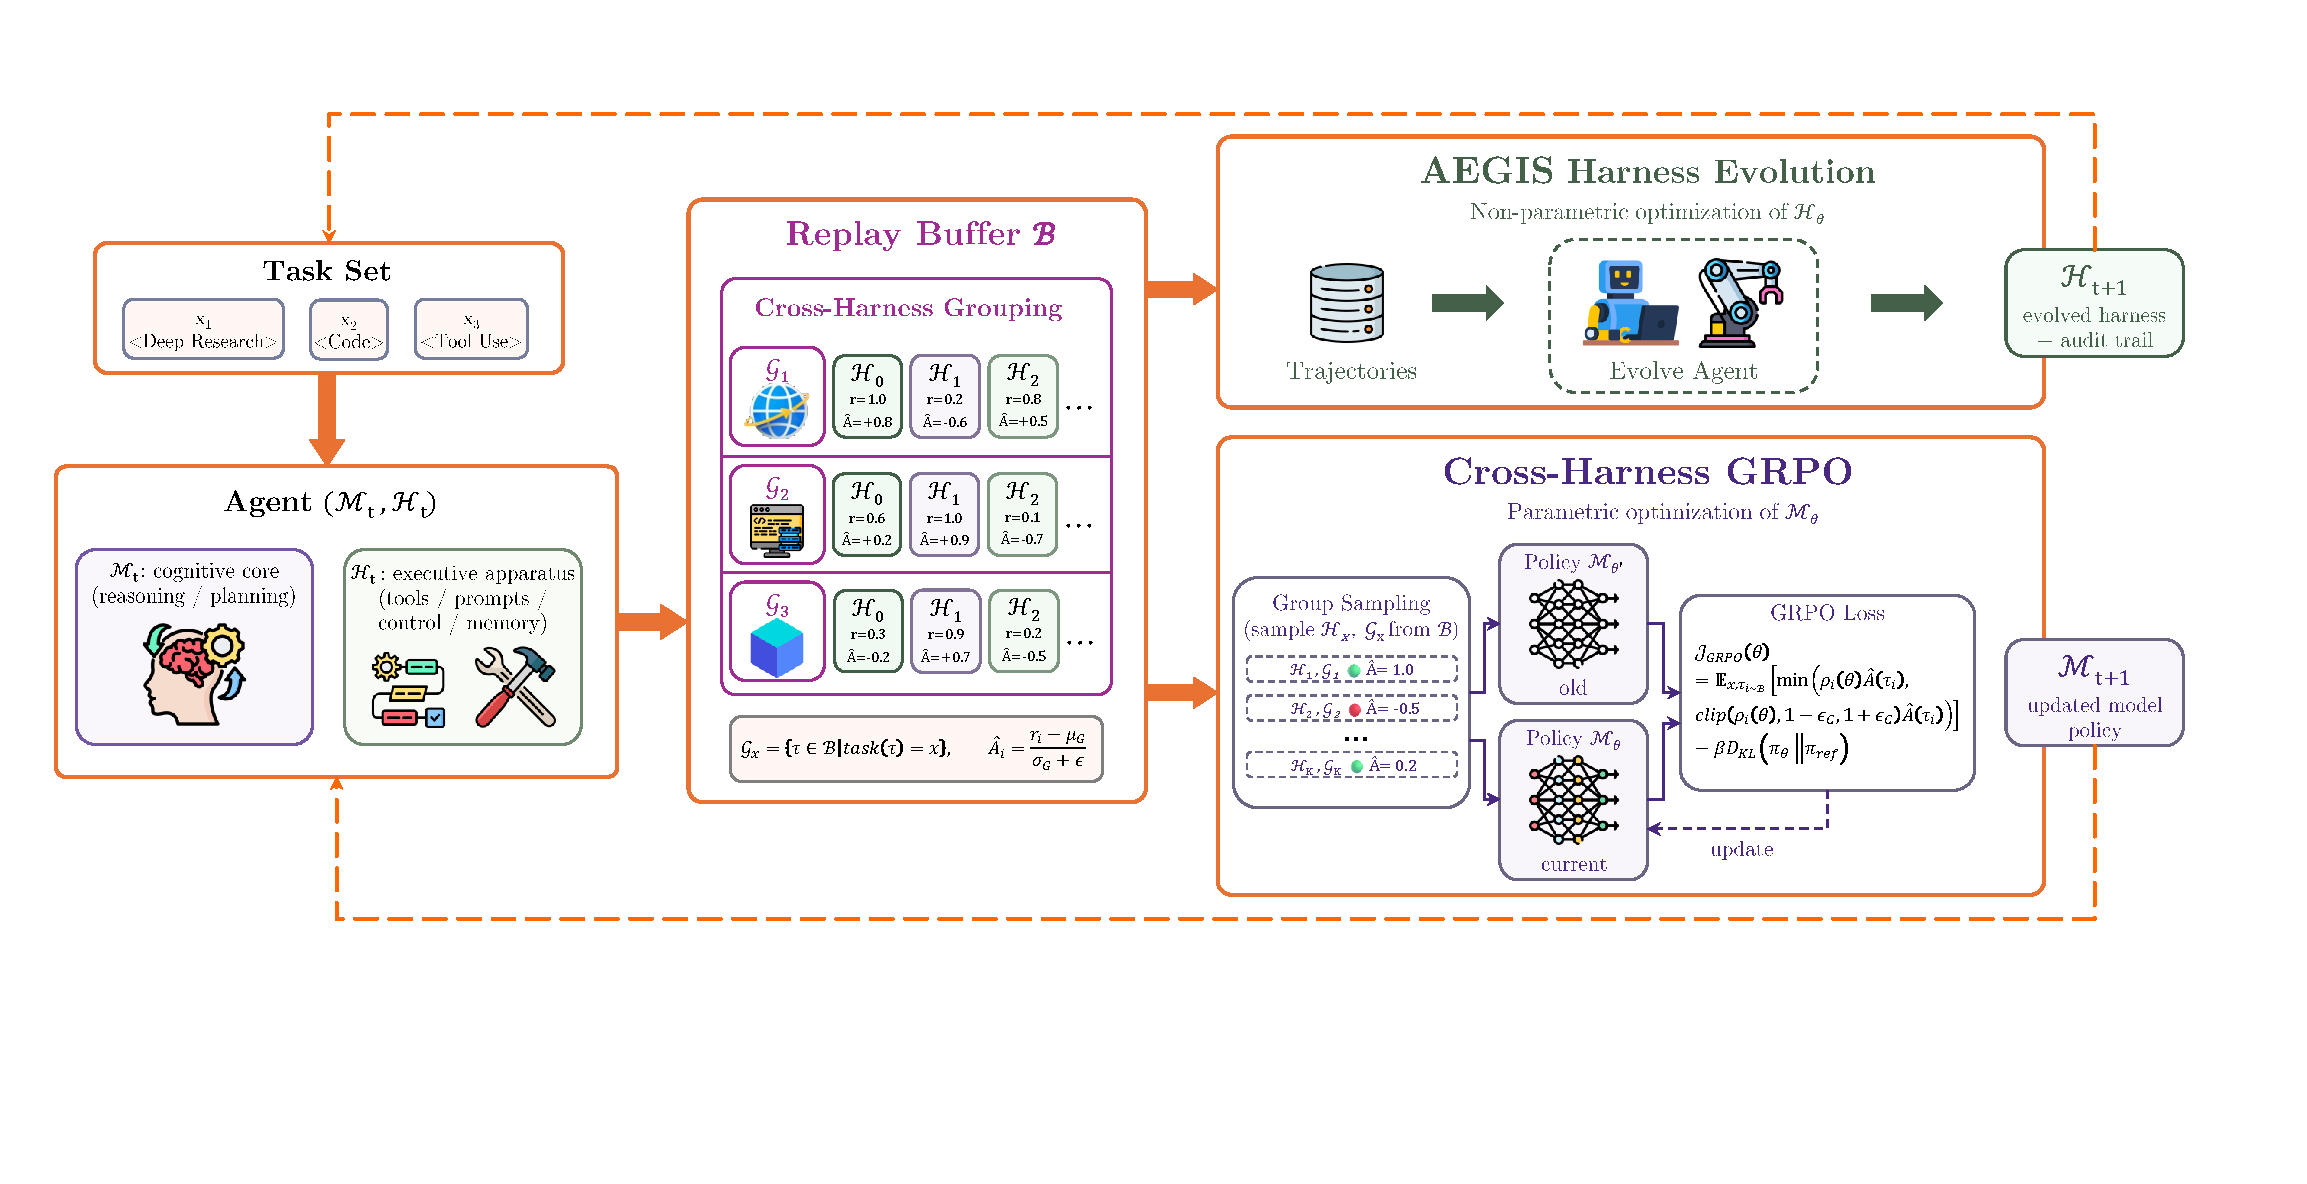
\includegraphics[width=\textwidth]{images/co-evo.pdf}
  \caption{\textbf{The harness-model co-evolution loop.} The agent $(\mathcal{M}_t,\mathcal{H}_t)$ runs the task batch $B_t$ under a fixed verifier and the observability layer; the resulting traces and rewards $(\tau,r)$ enter a shared replay buffer $\mathcal{B}$, where cross-harness grouping pools trajectories of the same task across harness versions and computes group-relative advantages $\hat{A}$. The same buffer drives two updates over identical data: AEGIS harness evolution (Digester $\to$ Planner $\to$ Evolver $\to$ Critic, yielding the evolved harness $\mathcal{H}_{t+1}$) and \textbf{cross-harness GRPO} (group sampling and a clipped GRPO objective, yielding the updated model $\mathcal{M}_{t+1}$); both feed the next iteration.}
  \label{fig:coevolution-loop}
\end{figure*}

\subsection{The Co-evolution Iteration}
\label{sec:coevolution-loop}

Co-evolution operates over the pair $(\mathcal{M}_t, \mathcal{H}_t)$, where $\mathcal{M}_t$ denotes trainable model parameters (relaxing the frozen-model assumption of Section~\ref{sec:method-aegis}) and $\mathcal{H}_t$ denotes the harness configuration at iteration $t$. The system maintains a fixed-capacity replay buffer $\mathcal{B}$ with first-in-first-out eviction. Each iteration proceeds as:

\begin{enumerate}[leftmargin=*]
  \item \textbf{Rollout.} Run $(\mathcal{M}_t, \mathcal{H}_t)$ on the adaptation batch $B_t$; the observability layer records each episode as a complete trace $\tau_i$, capturing every model turn, tool call, and tool result.

  \item \textbf{Verification.} A fixed verifier scores each trace into a scalar reward $r_i$. Holding the verifier fixed keeps rewards comparable across harness versions, which the cross-harness advantage (Eq.~\ref{eq:grpo-advantage}) requires.

  \item \textbf{Buffer insertion.} Append each scored trace to the shared buffer $\mathcal{B}$ together with the harness version that produced it, so successive rounds accumulate rather than overwrite; FIFO eviction keeps $\mathcal{B}$ restricted to recent rounds.

  \item \textbf{Harness evolution} ($\mathcal{H}_{t+1} \leftarrow \text{AEGIS}(\mathcal{H}_t, \mathcal{B})$, non-parametric, Section~\ref{sec:method-aegis}). The meta-agent reads the buffered traces as evidence of where the scaffold fails, proposes one discrete structural edit, and admits it only if the Critic and gating layer validate it.

  \item \textbf{Behavior log-probabilities.} For the traces just added this round, run a forward pass under the generating model $\mathcal{M}_t$ to obtain the token-level log-probabilities $\pi_{\theta_{\text{old}}}(\tau_i)$ and cache them for use in the GRPO loss; trajectories from earlier rounds reuse the values cached at their own insertion (Section~\ref{sec:coevolution-offpolicy}).

  \item \textbf{GRPO update} ($\mathcal{M}_{t+1} \leftarrow \text{GRPO}(\mathcal{M}_t, \mathcal{B})$, parametric, Section~\ref{sec:coevolution-grpo}). Partition traces into per-task groups spanning harness versions, assign each a group-relative advantage, and take a clipped policy-gradient step with a KL anchor to the fixed reference.

  \item \textbf{Advance.} Return to step~1 with the evolved pair $(\mathcal{M}_{t+1}, \mathcal{H}_{t+1})$.
\end{enumerate}

Every trace serves as both AEGIS diagnostic evidence and GRPO training signal. The harness evolution (step~4) and model update (steps~5--6) read the same buffer but neither conditions on the other's output within the same iteration; both must complete before the next rollout begins.


\subsection{Optimization Substrates}
\label{sec:coevolution-dual-grpo}

\paragraph{Harness side (non-parametric optimization).}
Harness evolution proceeds as in Section~\ref{sec:method-aegis}, drawing on the replay buffer $\mathcal{B}$ for trace evidence. The principal difference from standalone AEGIS is that $\mathcal{B}$ contains trajectories from multiple model checkpoints $\mathcal{M}_0, \mathcal{M}_1, \ldots, \mathcal{M}_t$, exposing the Digester to behavioral variation from both model updates and harness edits.

\paragraph{Model side (parametric optimization via GRPO).}
The key design choice is the \textit{cross-harness grouping criterion} (formalized in Section~\ref{sec:coevolution-grpo}): all trajectories sharing a task identifier form one GRPO group regardless of which harness or model checkpoint produced them, so that within-group variation reflects strategy differences rather than sampling noise alone.

\paragraph{Complementarity.}
The harness update makes discrete structural changes (adding a tool, replacing a control processor, restructuring the prompt) that cannot be expressed as parameter updates. The model update makes fine-grained behavioral adjustments (when to invoke which tool, how to phrase a query, when to terminate) that depend on high-dimensional in-context state and cannot be captured by symbolic specification. The harness defines coarse-grained strategy architecture; the model learns to exploit it.

\subsection{Model Training via Cross-Harness GRPO}
\label{sec:coevolution-grpo}

We adopt Group Relative Policy Optimization (GRPO)~\cite{shao2024deepseekmath}. Formally, each trajectory in the buffer is generated as:
\begin{equation}
    \tau_i \sim \text{Agent}(\mathcal{M}_k,\, \mathcal{H}_k,\, x_i), \quad k \in \{0, 1, \ldots, t\},
  \label{eq:trajectory-generation}
\end{equation}
where $i$ is the $(x, \tau)$ index in the buffer $\mathcal{B}$, $\mathcal{M}_k$ and $\mathcal{H}_k$ are the model checkpoint and harness used to roll out task $x_i$ into trajectory $\tau_i$. Because FIFO eviction bounds the buffer to recent iterations, buffered trajectories come from model versions close to the current policy. Yet they differ markedly in strategy (tool selection, prompt structure, control-flow logic), a diversity that stems from the successive harness versions $\mathcal{H}_0, \ldots, \mathcal{H}_t$. Unlike single-policy RL, where within-group variation reduces to stochastic sampling, here harness identity dominates that variation, which makes the cross-harness grouping criterion (Eq.~\ref{eq:cross-harness-group}) essential for meaningful advantage estimation.

Formally, for a task $x$, the trajectory group collects all traces of $x$ regardless of which $(\mathcal{M}_k, \mathcal{H}_k)$ pair produced them:
\begin{equation}
  \mathcal{G}_x = \{\tau_i \in \mathcal{B} \mid \text{task}(\tau_i) = x\} = \bigcup_{k} \{\tau \sim \text{Agent}(\mathcal{M}_k, \mathcal{H}_k, x)\}.
  \label{eq:cross-harness-group}
\end{equation}
The model therefore receives gradient signal from inter-strategy reward contrasts, rather than from stochastic variation within a fixed strategy alone, which enables it to internalize strategies that succeeded across harness versions.

\paragraph{Task-level alignment, not action-level.}
Cross-harness GRPO performs \textit{task-level} alignment: trajectories from different harness versions are grouped by task identity and compared by verifier reward alone. No action-level alignment is required, so harness versions with incompatible action spaces (different tool schemas, different prompt structures, different control-flow processors) coexist in the same group without conflict. When computing the policy gradient, each trajectory $\tau_i$ is replayed under the harness version $\mathcal{H}_k$ that produced it: the model's log-probabilities $\pi_\theta(\tau_i \mid x)$ are evaluated against the prompt, tool schema, and observation context that $\mathcal{H}_k$ would have constructed at each turn. The GRPO gradient thus operates entirely on model output tokens conditioned on harness-specific context, rather than on harness structural actions or environment transitions. This design decouples harness evolution (which may freely alter the action space across versions) from model training (which only requires token-level log-probabilities under each trajectory's own harness context).

The group-relative advantage is:
\begin{equation}
  \hat{A}(\tau_i) = \frac{r_i - \mu(\mathcal{G}_x)}{\sigma(\mathcal{G}_x) + \epsilon},
  \label{eq:grpo-advantage}
\end{equation}
where $r_i$ is the reward for trajectory $\tau_i$, and $\mu(\mathcal{G}_x)$, $\sigma(\mathcal{G}_x)$ are the within-group reward mean and standard deviation. The evolving harness acts as a structured exploration operator for the model's RL: each new version injects a distinct mode of behavior into the task's sampling distribution, and the advantage in Eq.~\ref{eq:grpo-advantage} commits the model toward whichever modes the verifier scores highest. The exploration breadth that single-policy sampling cannot provide is thus supplied by the evolving scaffold itself.

The policy objective to maximize is:
\begin{equation}
  \mathcal{J}_{\text{GRPO}}(\theta) = \mathbb{E}_{x,\, \tau_i \sim \mathcal{B}} \left[ \min\!\left( \rho_i(\theta)\,\hat{A}(\tau_i),\; \text{clip}\!\left(\rho_i(\theta),\, 1{-}\epsilon_c,\, 1{+}\epsilon_c\right)\hat{A}(\tau_i) \right) \right] - \beta\, D_{\text{KL}}\!\left(\pi_\theta \,\|\, \pi_{\text{ref}}\right),
  \label{eq:grpo-objective}
\end{equation}
where
\begin{equation}
  \rho_i(\theta) = \frac{\pi_\theta(\tau_i \mid x)}{\pi_{\theta_{\text{old}}}(\tau_i \mid x)}, \qquad \pi_{\theta_{\text{old}}} = \mathcal{M}_{d},
  \label{eq:grpo-ratio}
\end{equation}
is the importance-sampling ratio between the current policy $\mathcal{M}_{k}$ and the checkpoint $\mathcal{M}_{d}$ that generated $\tau_i$ (Eq.~\ref{eq:trajectory-generation}), $\epsilon_c$ is the clipping threshold, and $\beta\, D_{\text{KL}}(\pi_\theta \| \pi_{\text{ref}})$ penalizes divergence from the fixed reference model $\pi_{\text{ref}}$. The behavior policy $\pi_{\theta_{\text{old}}}$ in the ratio and the reference policy $\pi_{\text{ref}}$ in the KL term are distinct: $\pi_{\text{ref}} = \mathcal{M}_0$ is fixed throughout training, while $\pi_{\theta_{\text{old}}}$ varies per trajectory and must be recovered from the buffer (Section~\ref{sec:coevolution-offpolicy}).

\subsection{Off-Policy Training over a Mixed-Policy Buffer}
\label{sec:coevolution-offpolicy}

The replay buffer is intrinsically off-policy: at iteration $t$ it holds trajectories generated by checkpoints $\mathcal{M}_0, \mathcal{M}_1,\dots, \mathcal{M}_t$ under harnesses $\mathcal{H}_0, \mathcal{H}_1, \dots, \mathcal{H}_t$ (Eq.~\ref{eq:trajectory-generation}), so the buffer distribution does not match the policy $\pi_\theta$ under update. Recovering $\pi_{\theta_{\text{old}}}$ for each buffered trajectory is the central off-policy challenge.

\paragraph{Behavior policy $\pi_{\theta_{\text{old}}}$.}
The importance ratio (Eq.~\ref{eq:grpo-ratio}) corrects the gap between $\pi_\theta$ and the checkpoint $\mathcal{M}_{k}$ that produced $\tau_i$. Since $\mathcal{M}_{k}$ varies across the buffer, $\pi_{\theta_{\text{old}}}(\tau_i)$ cannot be recovered from any single model: we materialize it at buffer insertion via one forward pass under $\mathcal{M}_{k}$, cache the token-level log-probabilities on disk, and reuse them at every gradient step. This decouples the cached behavior log-probabilities from the current log-probabilities $\pi_\theta(\tau_i)$ recomputed each step.

\paragraph{Bounded off-policy bias.}
FIFO eviction caps the buffer at $C$ trajectories; with $s$ samples per round the maximum model-version lag is $\lfloor C/s \rfloor$ rounds, so every cached $\pi_{\theta_{\text{old}}}$ originates within a bounded window of $\pi_\theta$ and the policy that generated a trajectory never differs greatly from the one being updated. The same window bounds harness staleness, so the cross-harness groups (Eq.~\ref{eq:cross-harness-group}) mix only recent scaffold versions, and the model is never trained predominantly against an obsolete harness.

\paragraph{Replay reuse at no added rollout cost.}
The dominant cost of agentic RL is the rollout (executing the agent in the environment: model decoding, tool calls, and verification), not the gradient update. In co-evolution a single round of exploration produces one set of trajectories that serves both updates: the same traces drive the AEGIS harness update (Section~\ref{sec:method-aegis}) and, through the shared buffer (Section~\ref{sec:coevolution-loop}), the cross-harness GRPO model update. GRPO consumes these trajectories by replay and issues no rollouts of its own. The marginal cost of adding the model update is therefore confined to (i) one cached forward pass per trajectory to record $\pi_{\theta_{\text{old}}}$ and (ii) the gradient steps themselves, both of which are rollout-free. No trajectory is generated solely to train the model. Joint optimization is therefore economical: it buys model improvement for the price of offline training compute alone, without any rollouts beyond those harness evolution already performs.
